\documentclass[10pt,twocolumn,letterpaper]{article}

\usepackage{cvpr}
\usepackage{times}
\usepackage{epsfig}
\usepackage{graphicx}
\usepackage{amsmath}
\usepackage{amssymb}
\usepackage{svg}

\usepackage{mathrsfs}

\usepackage{cite}
\graphicspath{ {images/} }
% Include other packages here, before hyperref.

% If you comment hyperref and then uncomment it, you should delete
% egpaper.aux before re-running latex.  (Or just hit 'q' on the first latex
% run, let it finish, and you should be clear).
\usepackage[breaklinks=true,bookmarks=false]{hyperref}

\cvprfinalcopy % *** Uncomment this line for the final submission

\def\cvprPaperID{****} % *** Enter the CVPR Paper ID here
\def\httilde{\mbox{\tt\raisebox{-.5ex}{\symbol{126}}}}

% Pages are numbered in submission mode, and unnumbered in camera-ready
%\ifcvprfinal\pagestyle{empty}\fi
\setcounter{page}{1}
\begin{document}

%%%%%%%%% TITLE
\title{Improving BERT text generation with an Attention sampling method}

\author{\IEEEauthorblockN{ Juan Jose \\ Marquez Villacís}\\
\IEEEauthorblockA{
Politecnico di Torino \\
S287313@studenti.polito.it}
\and
\IEEEauthorblockN{Fabio Caffaro}\\
\IEEEauthorblockA{
Politecnico di Torino \\
S276842@studenti.polito.it}
\and
\IEEEauthorblockN{Yhorman Bedoya}\\
\IEEEauthorblockA{
Politecnico di Torino \\
S287296@studenti.polito.it}
}

\maketitle
%\thispagestyle{empty}

%%%%%%%%% ABSTRACT
\begin{abstract}
In this project, we developed a user-friendly interface making it easier
to experiment text generation with BERT. we introduced a new sampling method
that uses the information generated by the attention mechanism of BERT to decrease
the number of iterations necessary until convergence. we implemented a fine-tuning
method to train and generate text with a given structure and with a given sentiment.
the fine-tuning method is accompanied by a formatter class that helps the user to
structure the generations. we have made several experiments to test the performance of
our contributions.
\end{abstract}

%%%%%%%%% BODY TEXT
\section{Introduction}

In recent years, the field of text generation has become an ever-growing interest
with the advent of new methods for generating text. Pre-trained language models
such as BERT have been used for a variety of NLP tasks. Taking advantage of BERT’s
MML task, \cite{wang2019bert} has proposed to use BERT as a text generator. In this project,
we analyse the ways in which BERT can generate sentences by taking advantage of its
architecture. Firstly, we describe three steps for the generation process: initialization,
sampling and replacement. Within this process we propose a different approach for the
sampling part, utilizing BERT’s attention mechanism to select at each iteration the most
appropriate tokens to be replaced by the model. A penalised attention mechanism is
introduced to overcome the difficulties of the model to select some tokens more frequently
than others for replacement.

Having a working BERT-based model to generate text we perform a fine-tuning of the model
to extend its abilities to generate Italian text. In this way, it was possible to have the
model learn the structure of Italian poetry, generate tweets and motivational quotes.
Another proposal on how to extend the model abilities, consist of adapting the model in
the training phase so that it can generate text according to a specified sentiment
(e.g., generate positive tweets).

The evaluation of machine generate text is a complicated task, having different metrics
to represent the goodness of the writing. In this work, we compare the results of the Bleu
score with the results of \cite{wang2019bert} and discuss the efficiency of the introduced attention
mechanism.

%-------------------------------------------------------------------------
\section{Current methods}

In recent years, the field of Natural Language Generation (NLG) has expanded its repertoire
of solutions for text generation to include a variety of methods.
Models such as RNN's, Bi-LSTM, Transformers-based models (e.g., GPT), GAN's, among others, have evolved
to produce elaborate pieces of text for different specifics tasks.
Each method proposes a different approach to the task at hand.

\subsection{RNN}

Recurrent Neural Networks (RNN) are commonly used in sequence-to-sequence (seq2seq) tasks, such as text generation.
Simple RNN's have been adapted to overcome its own limitations, e.g., vanishing or exploding gradients,
introducing concepts such as Long Short Term Memory networks (LSTM) or even bidirectional LSTM's (Bi-LSTM).
LSTM's and Bi-LSTM have been used in many cases for text generation \cite{Bengali} \cite{lstm1} \cite{lstm2} \cite{lstm3}.
These models are still used in recent years.
Some studies \cite{embedds} use external word embeddings for the training process which can be seen as pre-trained
models for text generation.

In this work, we train a simple RNN with an Embedding layer, one LSTM module and a dense output layer.
The task of the RNN is to predict the next word for the text generation.
For this net, several hyperparameters can be set such as the number of LSTM layers, whether those layers
are bidirectional, pre-trained word embeddings, among many others.
The configuration that best minimized the cross-entropy loss was an embedding layer with no pre-trained embeddings,
three bidirectional LSTM layers and one dense output layer.
With this configuration, 1000 sentences were generated for comparison with alternative methods.

\subsection{Transformers}

With the introduction of \cite{attention}, new models for text generations task have arisen.
\cite{attention} introduces an Encoder-Decoder based architecture for machine translation tasks.
This architecture was ingeniously modified by \cite{bert} and \cite{gpt} to yield models such as BERT and GPT.
Both Generative Pre-trained Transformer (GPT) and Bidirectional Encoder Representations from Transformers (BERT)
are based on the idea of transformers and can be finetuned and
adapted for a variety of tasks \cite{gptapps1} \cite{gptapps2} \cite{gptapps3} \cite{gptapps4} \cite{gptapps5}.
These models have slowly replaced the RNN approaches.
As \cite{modernMethods} states: "Transformers disrupted sequence-based deep learning significantly.
The two variants of transformer models that we showed, BERT and GPT-2, outperform
previous approaches with RNNs".

GPT is widely known as a powerful tool for text generation.
Conversely, the BERT model alone has not been accepted as a strong generative model.
Some authors \cite{wang2019bert} have proposed workarounds to BERT limitations for text generation.

%------------------------------------------------------------------------
\begin{figure*}[t]
   \centering
   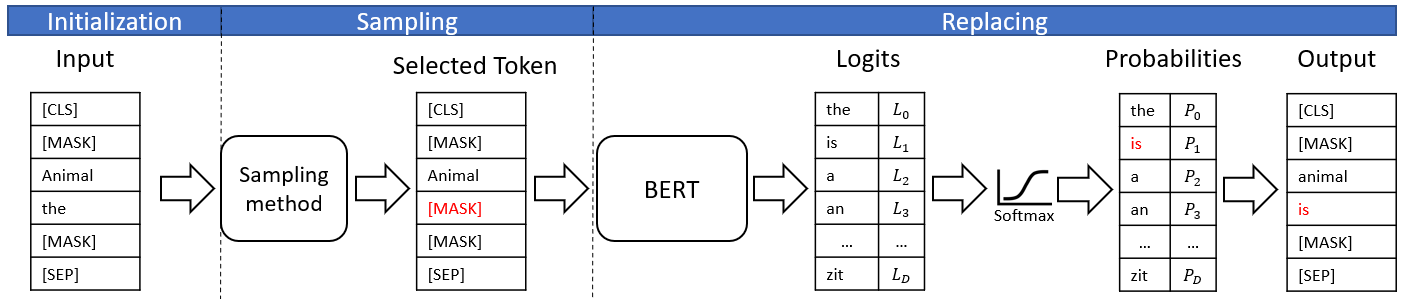
\includegraphics[scale=0.6]{BERTfunc.PNG}
   \caption{Process to use BERT as a generator.}
   \label{fig:BertFig}
\end{figure*}

\section{BertTextGenerator}
BERT is a language representation model designed to achieve state-of-art results
in several natural language processing tasks such as question answering and language inference.
BERT is trained on masked language modelling objective, in which it predicts a word given its
left and right context.
Given this behaviour, it is possible to deduct that BERT is not the most
indicated model for text generation tasks.
However, \cite{wang2019bert} have demonstrated why it is possible to use BERT as a traditional
language model by means of showing that BERT is a combination of a 'Markov random field
language model (MRF-LM), with pseudo Log-Likelihood training'.
This conclusion allows using BERT as a generative model of sentences to either score a sentence or
sample a sentence.

To generate text with BERT the process is composed by 3 main steps described as follows and illustrated in the Figure \ref{fig:BertFig}:

\begin{itemize}
\item Initialization: It is necessary to initialize the sequence with a random initial state, this can be either an all-mask sequence,
i.e., [MASK], ..., [MASK], an all-random sequence, or a combination of these, i.e. 50\% [MASK] tokens and 50\% random tokens.
\item Sampling: At each iteration, it is necessary to choose which token of the sequence will be masked, in \cite{wang2019bert}
they propose the Sequential sampling in which the sequence is masked from left to right one token at a time at each iteration,
and the Parallel sequential sampling in which the sequence is masked choosing at random one token at each iteration.
\item Replacement: Finally, the sequence with the masked token is passed to BERT to produce a tensor of logits $L$ of
the length of its vocabulary $v (v \approx 30K)$. Those are interpreted as the probability of the token to be present in the current sequence.
Finally, the logits are normalized using a SoftMax function to get a probability distribution and select the new token to be inserted.
\end{itemize}

The initialization is made only once at the beginning of the generation process, the sampling and the replacing are
made once for each iteration of the model.

In \cite{wang2019bert} they use a set of parameters to set up the generations,
we add a new set of parameters to make easier the use of the model and
to include some new functionalities. We insert a way to
change the composition of the initial state with the parameter $init\_mask\_prob$.
We make easier to change the generation method with the parameter $generation\_method$.
We introduce a way to create sentences with different length in one generation with the parameters $Max\_len,
Min\_len, Avg\_len and Std\_len$. Finally, we add the possibility to mask and replace more
than one token for each sentence at each iteration with the parameter $masked\_portion$.

%------------------------------------------------------------------------
\subsection{Attention mechanism}
The attention mechanism is composed by a feed forward neural network that is trained to
identify the more relevant components in the context in order to predict a new token.

For example, take the sentence "the animal didn't cross the street because it was too tired",
as a human it is easy to know that in the sentence the pronoun "it" refers to the subject "the animal"
and the verb "was" is the correct conjugation of the verb "To be" for the third person, but for an
algorithm is not easy to know these relationships and that is the task of the attention mechanism.
Considering the same sentence
some attention heads would focus on the verb "was", other attention heads would focus
on the special tokens "[CLS]" and "[SEP]" that represent the beginning and the end of the sentence
respectively, finally other attention heads would focus on the word "animal". In this way BERT can
understand which parts of the context are more relevant.

\subsubsection{Using the attention mechanism to improve the sampling method.}
When a token is predicted, it is possible to know which tokens of the context were more relevant to
retrieve the prediction based on the attention weights.
This information is a meaningful insight to improve
the way in which the sampling method is made.

We propose a new sampling method based on the attention
weights returned by BERT when a prediction is done.

\paragraph{Attention based sampling}
First, we design a sampling method totally based on the attention weights, when a token is replaced we retrieve
and summarize the attention information corresponded to the replaced token using averages inside and between the
encoders to get a unique measure of the attention, then we normalize the result to get a probabilistic interpretation
and we make the new sample based on this probability, in this way we wanted to sample the more related tokens to the one
that was already replaced to check if these tokens preserve his meaning in the sequence.

However, we found that the attention mechanism creates very strong correlations between
few tokens of the sequence, then the sample got stuck always choosing the same tokens among
all the iterations.
To solve this behaviour, we add a penalization to those tokens that were
chosen several times, in the next section we describe the new method.

\begin{figure}
   \centering
   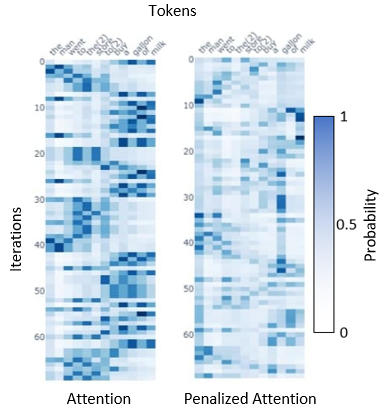
\includegraphics[scale=0.7]{attComp.PNG}
   \caption{Comparison of the behaviour of the proposed sampling methods.}
   \label{fig:AttentComp}
\end{figure}

\paragraph{Penalized attention sampling}
This method is very similar to the previous one, however, we include a penalization factor
to those tokens that were chosen several times, in that way the sampling method makes a better
exploration of the sequence based on the attention information and as a result we get better
generations.

To carry it out we retrieve the attention masks of the iteration $t-1$ ($a$), then get the average value of
the attention masks ($A_{p,e}$) for each position $p$ inside each one of the encoders $e$. subsequently, we get
the average value of the attention masks ($totalA_{p}$) for each position over all the encoders.
In this way, we reach to summarize all the attention information in only one tensor.
afterward, for each position $p$, we set a counter $c$ that registers how many times the position $p$ has been selected to be replaced.
Next, we divide the average value of the attention masks ($totalA_{p}$) by the counter $c$.
This step is useful to avoid that the sampling method gets stuck sampling always the same positions.
Finally, we normalize the result to get a probability distribution $P$ and we sample randomly from it the new token to be replaced.

In the Figure \ref{fig:AttentComp} it is possible to see how the probability of choose a token evolves
during the iterations, it is possible to note how the attention method
get stuck during several iterations in the same areas of the sequence, for example, during the iterations
10 to 16, the probability was focus on the last 4 tokens of the sequence.
While in the penalized attention is possible to see a more balance probability distribution inside each iteration
and the sampling method is not focus on only few parts of the sequence.
%------------------------------------------------------------------------
\subsection{Finetuning}
BERT is a powerful model pre-trained on a broad set of text composed by the whole
BooksCorpus and Wikipedia corpora \cite{wang2019bert}.
One of its main features is its adaptability to a plethora of different tasks,
by means of a fine-tuning on specific domain set.
Typical fine-tuning techniques depend on the final task that the user requires BERT to perform.
For example, considering classification tasks such as sentiment prediction and text classification,
the fine-tuning will be focused on the [CLS] token, a special token used in the pre-training
phase for the task of \textit{next-sentence-prediction} and specifically designed for classification applications.

Text generation is not a usual task for BERT.
In this case, the fine-tuning aims to make the model understand the structure of the text,
in order to mimic it at inference time.
We have implemented a fine-tuning procedure that relies on a \textit{Cloze} task, similar to the one adopted also in the
 original training \cite{bert}.
This consists of replacing a percentage (15\% by default) of the tokens for each sentence with a [MASK] token and let
BERT predict the blanks. The logits outputted by the model are then used to compute the cross-entropy
loss with respect to the original token that were replaced.

This method allows the final user to start from a pretrained model and fine-tune it on a specific
text corpus in order then to make it generate text similar to the original one.
This approach also works in the case that a pretrained model is not available in the language selected by the user.
In this case, the user can simply start from a Multilingual Models and applying a process referred to as 
Cross-Lingual Transfer Learning\cite{crosslanguage}.

\subsubsection{Structure of the text}
\label{section:structureText}
The default vocabulary of the tokenizer contains around 1000 unused tokens, whose weights are randomly initialized.
Typically, these tokens are replaced with domain specific words, so that during the fine-tuning phase
the model will be able to learn their representation.
We have extended this idea in order to comprehend also tokens that define the structure of the text like
'\textbackslash n' and '\textbackslash t'.
Note that, simply adding these tokens to the vocabulary would have no effect.
These tokens in fact, are typically replaced even before the tokenization, during the normalization step of the tokenization pipeline.

However, these tokens can be fundamental, especially in the task of text generation.
To solve this problem, we have implemented a Formatter class that helps the user to format the text in order
to preserve the important tokens.
The Formatter replaces a user specified set of tokens that need to be preserved, with some unused tokens.
The replacement happens before the tokenization, in this manner, during the fine-tuning the model will be able to learn
the position of these important tokens.
The unused tokens are then replaced back with the original ones after the generation.

Using this method, we were able to fine-tune a model able to learn the famous tercet structure of Dante's Divine Comedy.

\subsubsection{Sentiment generation}
\label{sentiment}
An important aspect of BERT tokenizer are special tokens like [CLS], [MASK] and [SEP].
As the name suggests, these are tokens with special functions.
The tokenizer gave the possibility to define new special tokens.
We have taken advantage of this opportunity to define a new method to generate text with a specific sentiment or label.

Consider a domain set $\mathcal S$ of sentences each one with an attached label $y\in \mathcal Y$,
i.e.\ a text whose label-set are the two possible sentiments $\mathcal Y =\{pos, neg\}$.
The method consists of three main steps:

\begin{itemize}
\item For each sentiment in the label set $y\in\mathcal Y$, we define $n$ (3 by default) special tokens $[y_i]\;\; for\;\;i=1,\ldots n$.
In the case of $y=pos$ for example the set of special tokens will be $\{\text{[pos-1]}, \text{[pos-2]}, \text{[pos-3]}\}$
\item Before the fine-tuning each sentence $s\in\mathcal S$ is tokenized, and the special tokens corresponding to its label are appended at the beginning of the list of tokens.
\item The fine-tuning is performed. During this step the model will build a relation among the special tokens of a sentiment and the specific words
related to it.
\end{itemize}
To generate the text with a given sentiment, the special tokens related to that sentiment are used as a seed to create
a context on top of which BERT can start to generate.
$$\big[     \text{[CLS]}\quad\underbrace{ \;\; \text{[pos-1]} \;\; \text{[pos-2]} \;\; \text{[pos-3]}}_{seed}
      \quad      \text{[MASK]} \quad\text{[MASK]}\quad\ldots$$

This method, even in its simplicity, showed its efficacy in generating positive and negative Italian tweets about football.
In addition, this method will allow the possibility to consider even more than two labels.
%------------------------------------------------------------------------
\begin{table}
\centering
\begin{tabular}{lllll}
\hline
\multicolumn{1}{c}{}                            & \multicolumn{4}{c}{\vcell{Model}}                  \\[-\rowheight]
\cline{2-5}
\multicolumn{1}{c}{\multirow{}{}{Parameter}}                           & \begin{tabular}[c]{@{}l@{}}Parallel\\ 1\end{tabular} & \begin{tabular}[c]{@{}l@{}}Parallel\\ 0.15\end{tabular} & Sequential & Attention  \\
\hline
%Avg\_len                                       & 40        & 40           & 40         & 40         \\
Std\_len                                       & 5         & 0            & 5          & 0          \\
Masked\_p                                      & 1         & 0.15         & 1          & 1          \\
%Sample                                         & True      & True         & True       & True       \\
Init\_mask\_p                                  & 1         & 1            & 0          & 1          \\
%Temperature                                    & 1         & 1            & 1          & 1          \\
Top\_k                                         & 0         & 100          & 100        & 100        \\
Iterations                                         & 500         & 500          & 500        & 200        \\
\hline
\end{tabular}
\caption{Parameters configuration of the best models obtained for each generation method.}
\label{tab:parameters}
\end{table}



\begin{table}[]
\begin{tabular}{lllll}
\hline
\multicolumn{1}{c}{} & \multicolumn{2}{c}{Bleu} & \multicolumn{1}{c}{\multirow{}{}{}} & \multicolumn{1}{c}{} \\ \cline{2-3}
\multicolumn{1}{c}{\multirow{}{}{Model}}   & WT103       & TBC        & \multicolumn{1}{c}{\multirow{}{}{Perplexity}} & Self-Bleu  \\ \hline
Original \cite{wang2019bert}                & 7.06        & 7.8        & 279.1        & 10.06                                            \\
Original*                            & 6.86        & 7.14        & 270.6             & 8.43                                  \\
Parallel-1                                 & 6.62        & 7.21       & 287.6                    & 6.83                           \\
Attention                                 & 8.15        & 6.59       & 386.6                  &  11.88                          \\
Parallel-0.15                              & 8.79            & 7.11           & 1241         & 12.02                                       \\
Sequential                                & 5.73            & 7.27           & 374.2          & 7.05                                      \\
RNN (WT)                                & 8.54            & 2.9           & -                  & 15.23                              \\
RNN (TBC)                                & 5.73            & 7.27           & -                & 7.45                                \\ \hline
\end{tabular}
\caption{Quality and diversity metrics of model generations.}
\label{tab:results}
\end{table}

\section{Experiments and evaluation}

The evaluation of generated text is not a simple task.
Some evaluations rely on intrinsic or extrinsic techniques.
Within these techniques metrics such as n-gram overlap metrics (f-score, bleu, self-bleu, rouge, meteor),
distance-based metrics, diversity metrics, content overlap metrics or even grammatical feature based
are considered.
Each metric reflects different results.
For example, the self-bleu represents the diversity of the text \cite{texygen}.
But this metrics are not perfect and can also be deceived.
\cite{evaltextgen1} explains the different struggles these measures have.
For example, it states that "a language model optimized only for perplexity
may generate coherent but bland responses."
In this sense, it is not simple to evaluate a text generator model based on a single metric.

% Grid search explanation
% Best model 1000 sents
% Corpus Bleu, perplexity and rouge
% Self-Bleu and n-Grams

We have made a Grid Search to analyse the behaviour of the generations and to identify the best combination of parameters for each one of the sampling methods.
For each one of the different combinations of parameters we have made five different generations each one with 50 text lines,
then we calculated different measures to analyse the quality and the diversity of the generations like
Bleu on Wikitex-103 (WT103) and TBC using the Texygen library \cite{texygen}, rouge and \%Unique N-grams. We select the three best models for each
generation method. Finally, we generated 1000 text lines with each one
of the selected models, we evaluate the final generations and based on the results we choose the best combination of
parameters for each generation method, in table \ref{tab:parameters} we report the obtained results.

In table \ref{tab:parameters}, we report the Bleu scores with respect to WT103 and TBC for the best models we found,
the results reported on \cite{wang2019bert} and its corresponding using Texygen as evaluator, and our RNN trained on WT103.5 and TBC.
It is possible to note that the proposed attention method is very near of the base line marked by \cite{wang2019bert},
even outperforming the base line in the Bleu measure with respect to WT103.


%---------------------------------------------------------------------------------------------
\subsection{Convergence of the attention sampling method}
As showed in \ref{tab:results}, the penalized attention method required less than a half
of the iterations with respect to the other methods, to reach similar results.
To analyse further this behaviour, we have made an experiment measuring the average number
of iterations needed to replace all the starting [MASK] tokens \ref{fig:ReplaceMask}.
This is an indicator of the speed at which the method can create a context for the sentence.
The parallel and the vanilla attention methods, required in average more than 80 over 150 iterations.
This means that the model had less than 70 remaining iterations to try to replace tokens with a complete sentence.
Moreover, they showed a very high variability.
On the other hand, the penalized attention method showed a much faster replacement with a lower variability.

\begin{figure}[t!]
   \centering
   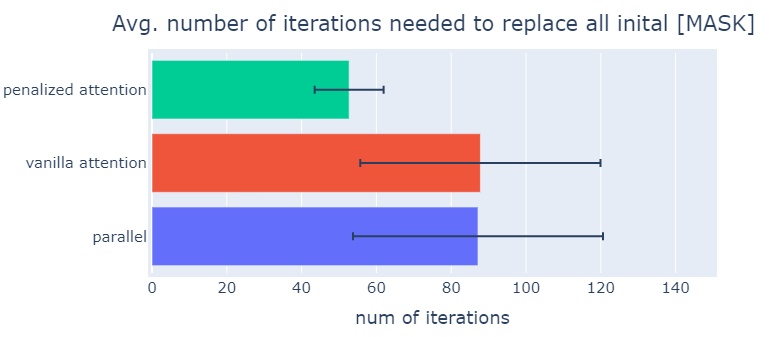
\includegraphics[width =\linewidth]{newplot (21).png}
   \caption{Average number of iterations needed to replace all the original [MASK] tokens.
   The experiment was performed on 80 generations for each method, each one with 150 iterations.
   The sentences were initialized as a list of 25 [MASK] tokens.}
   \label{fig:ReplaceMask}
\end{figure}

This behaviour reflects on a faster convergence of this method.
In \ref{fig:Recall} we have plotted the average recall score for unigrams and bigrams during the iterations.
All the methods were reaching a similar plateau, with a drastic change of slope in correspondence of the
average number of iterations needed to replace the masked tokens. The penalized attention mechanism was clearly the
one able to reach it faster.

\begin{figure}[t!]
   \centering
   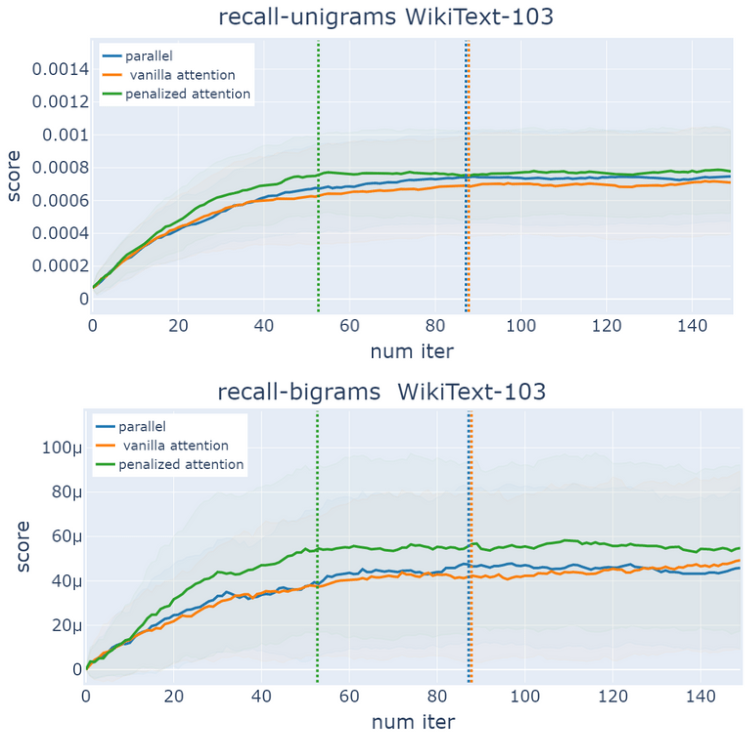
\includegraphics[width=\linewidth]{recall.png}
   \caption{Average recall score of unigrams and bigrams w.r.t WikiText-103
   at each iteration. The dashed lines correspond to the avg num of iterations needed
   to replace the initial mask tokens}
   \label{fig:Recall}
\end{figure}

\subsection{Italian generation: finetuning experiments}
In order to test the functionality of the fine-tuning we have performed three experiments
\footnote[1]{https://github.com/JuanJoseMV/neuraltextgen/blob/main/Example\_finetuning.ipynb}.
All the experiments were performed with an Italian pretrained BERT model
\footnote[2]{https://huggingface.co/dbmdz/bert-base-italian-cased}
applied on Italian sets of text.
All the fine-tunings use the AdamW optimizer with linear schedule with warmup, as common use for finetuning transformer methods.

\paragraph{Motivational quotes} In the first experiment we have gathered a small set of motivational quotes,
constructed scraping from different sources. The quotes were pre-processed in order to make them
all structured in the same way:
\begin{quote}
   A motivational quote - (anonymous)
\end{quote}

The model was finetuned for 4 epochs with starting $lr=5e^{-5}$. The results were quite surprising,
the model was able to learn the structure of the quote and to generate some meaningful text.
This is an example:

\begin{quote}
non hai nulla da fare, tutti i giorni, se non stai cercando di fare tutto cio che e necessario. ( norman bates )
\end{quote}

%\begin{quote}
%   se vuoi davvero fare una cosa, e meglio se la smetti di farla. ( thomas edison )
%\end{quote}
Obviously not all the quotes were this good.
A lot of generations were stuck on repetitions of the same words or tokens.
This is a common problem that we have found on all the generations with BERT that we have done.
The sampling methods that outputted the most reliable quotes seemed to be the penalized attention and the sequential.

\paragraph{Dante's divine comedy} The second experiment was focused on the structure of the text,
for this part we have used Dante's Divine Comedy
%\footnote[1]{https://github.com/dlang/druntime/blob/master/benchmark/extra-files/dante.txt}.
The model was fine-tuned on tercets (groups of three lines) instead of single lines.
\begin{quote}
   Nel mezzo del cammin di nostra vita\\
   mi ritrovai per una selva oscura,\\
   ché la diritta via era smarrita.\\
\end{quote}
Each tercet was pre-processed replacing '\textbackslash n' with 'unused1' tokens as explained in \ref{section:structureText}.
Also in this case, the model was finetuned for 4 epochs with starting $lr=5e^{-5}$. These are 2 tercets generated:
%\begin{quote} %['Nel', 'mezzo', 'del', 'cammin', 'di', 'nostra', 'vita', \textbf{'unused1'}, % 'mi', % 'ritrovai', % 'per', \ldots%% 'una',%% 'selva',
%% 'oscura,', %% \textbf{'unused1'}, %% 'ché',%% 'la',%% 'diritta',%% 'via',%% 'era',%% 'smarrita.',%% \textbf{'unused1'}]%\end{quote}

\begin{quote}
% che mai non m ’ io coglia ;\\
% e non abbracci che li si ridesse,\\
% che piu tempo fece prodente.\\
%
%
% ma vidi io di lo vento che\\
% del son s ’ accesi io :\\
% per tanto piacer che questo venisse il triscio ».\\
sappi pero che la tua mente e buona,\\
che si fa la volonta di dio,\\
com ’ e stata fatta l ’ arte del mondo,\\

“ e ’ l viso mio “ chinato ”,\\
e ’ l vidi correr dietro a me\\
si tentenno e disse : « loco, loco! ».\\
%
% ma gia di queste le zanne\\
% sonn piu, si malicce,\\
% che prima l ’ occhio non era in ciel ;\\
\end{quote}

%\begin{quote}
%
%e disse a me : ‘ e tu? ’\\
%piu in la che vidi, piu non si facea ;\\
%questo e ’ l padre mio, che e con me ».\\
%
%e cato e cato, e in lui\\
%si fece ’ l uno e un altro,\\
%si che ’ l le membra e lo spirito movea ».\\
%
%sappi pero che la tua mente e buona,\\
%che si fa la volonta di dio,\\
%com ’ e stata fatta l ’ arte del mondo,\\
%che non e morta.\\
%
%“ e ’ l viso mio “ chinato ”,\\
%e ’ l vidi correr dietro a me\\
%si tentenno e disse : « loco, loco! ».\\
%\end{quote}

All the '\textbackslash n' tokens present in the quote were automatically generated by the model.
Also in this case the attention sampling method seemed the one able to reproduce the structure in the most reliable way.


\paragraph{Sentiment generation} In this case we have used a dataset
composed by 12000 Italian tweets extracted from
\footnote[1]{https://github.com/charlesmalafosse/open-dataset-for-sentiment-analysis}.
Each tweet with one of 4 possible sentiment labels
$\mathcal Y = \{\text{POSITIVE}, \text{NEGATIVE}, \text{MIXED}, \text{NEUTRAL}\}$.
The dataset was highly imbalanced with respect to the last two classes, so we have considered only the first two
selecting 6000 tweets for each one.
The dataset was pre-processed as explained in \ref{sentiment}; in addition, a set of tokens was added to the vocabulary
in order to deal with '@tags' and '#hashtags'. We have generated new tweets, setting [POSITIVE]/[NEGATIVE] + "Ronaldo", as starting seed:\\

[POSITIVE]:
\begin{quote}
   ronaldo tante complimenti per per il tuo bellissimo debutto, dopo aver visto il tuo punto forza e auguri @\_/juventusfc #juventusfc #juventusfc?
\end{quote}

[NEGATIVE]:
\begin{quote}
   ronaldo??? molto bene? molto bene??? non si vince mai con sportivita e fiducia non ti preoccupare hai dimostrato di non poter faticare a nulla
\end{quote}

Other example of the generations can be found on the Appendix \ref{sec:appendix}.

\section{Conclusions}
In this project we explored the usage of BERT as a text generator,
focusing in particular on the sampling part of the method.
Our new attention method was able to reach the results obtained in the original paper
improving the convergence time, and the number of iterations needed.

As in the original paper, the results of BLEU score on the generation of a wide body of text
showed the unreliability of BERT in text generation,
due to incapacity of controlling it.
In particular, a typical problem that we have encountered was that in
a considerable number of iterations the model was stuck in a bad part of the
configuration space i.e., all '.' tokens or repetition of groups of tokens.
The consequence was that BERT was keeping replacing the tokens with the same ones
until the last iteration.

Nonetheless, our experiments showed the possibility to still apply the model
on specific domains i.e, quotes, through a fine-tuning.
In this case, BERT were able to clearly understand
the structure and generate some meaningful text.

Due to high variability of the results, we can conclude that no sampling method was clearly
outperforming the others. This suggests the possibility of future exploration in other parts
of the generation method. In particular, it could be interesting a further investigation
of the resampling part and the implementation of a scheduling of the temperature of the logits,
in order to help the generation method to not get stuck in the early stages of the generation.

\bibliographystyle{ieeetr}
\bibliography{egbib}

\section*{Appendix}\label{sec:appendix}

%\begin{figure}
%\centering
%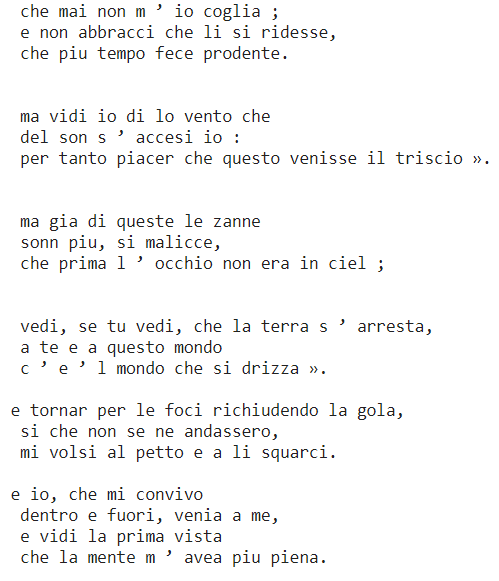
\includegraphics[width=\linewidth]{dante1.png}
%\caption{Average recall score of unigrams and bigrams w.r.t WikiText-103
%at each iteration. The dashed lines correspond to the avg num of iterations needed
%to replace the initial mask tokens}
%\label{fig:Recall}
%\end{figure}
%\begin{figure}
%\centering
%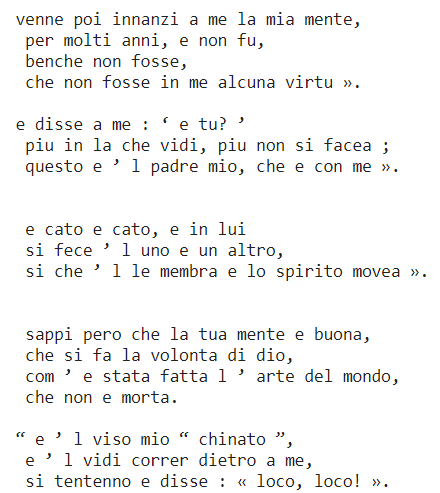
\includegraphics[width=\linewidth]{dante2.png}
%\caption{Average recall score of unigrams and bigrams w.r.t WikiText-103
%at each iteration. The dashed lines correspond to the avg num of iterations needed
%to replace the initial mask tokens}
%\label{fig:Recall}
%   \newpage
%\end{figure}
\begin{figure}[ht]
\centering
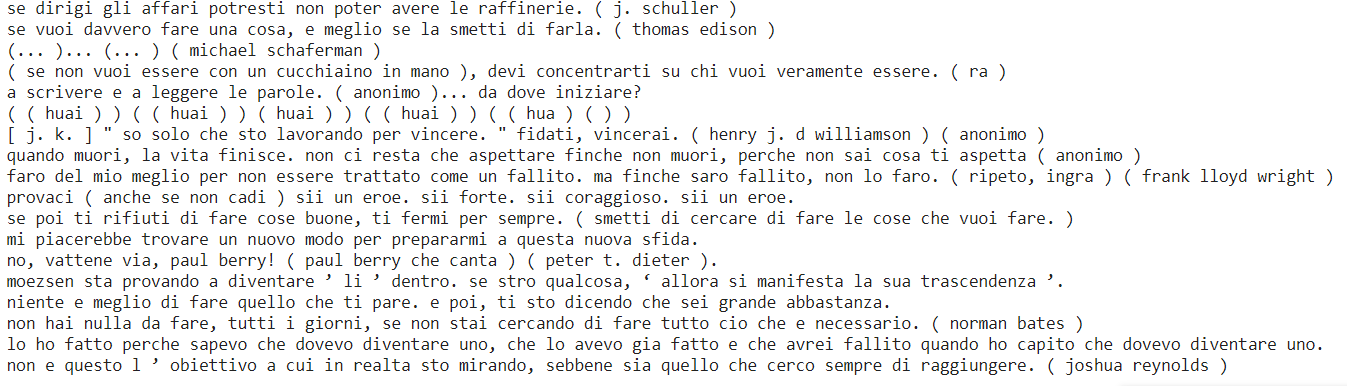
\includegraphics[width=\textwidth]{quotes.png}
\caption{Examples of generation of quotes from eperiment 1}
\end{figure}


\begin{figure}[ht]
\centering
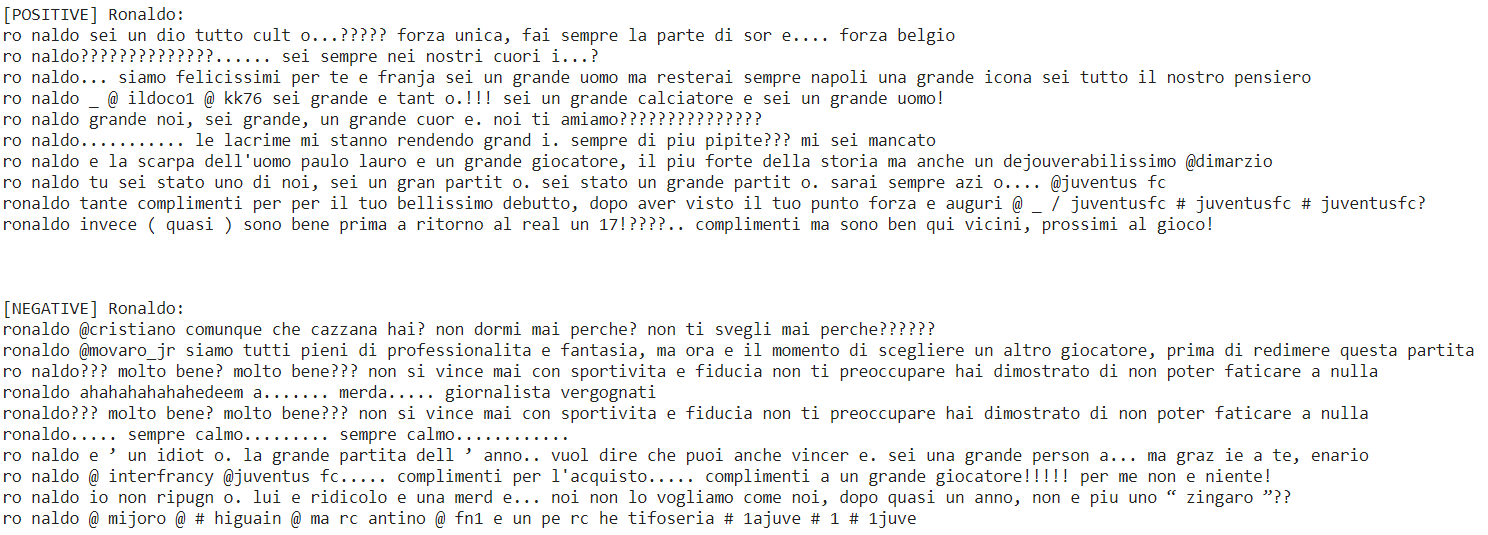
\includegraphics[width=\textwidth]{tweets.png}
\caption{Examples of generations of tweets with sentiment (3rd experiment). The tweets are separated by sentiment (POSITIVE/NEGATIVE).
In addition, for each sentence we used "Ronaldo" as seed to start the generation.
}
\label{fig:tweets}
\end{figure}
\clearpage
\mbox{~}


\begin{figure}[ht]
\centering
\begin{subfigure}{.5\linewidth}
  \centering
  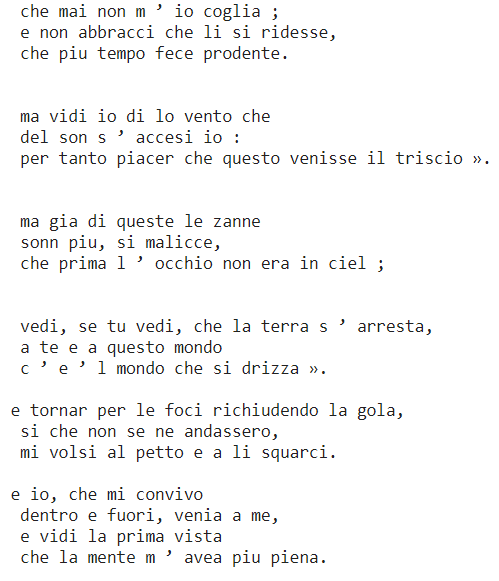
\includegraphics[width=\linewidth]{dante1.png}
  \label{fig:dante1}
\end{subfigure}%
\begin{subfigure}{.5\linewidth}
  \centering
  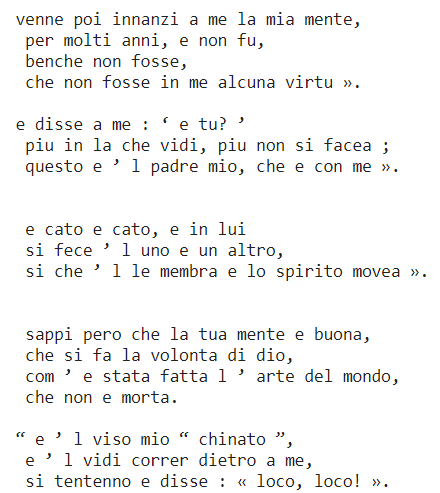
\includegraphics[width=\linewidth]{dante2.png}
  \label{fig:sub1}
\end{subfigure}%
\caption{Two examples of generation after fine-tuning the model on Dante's Divine Comedy, from experiment 2}
\label{fig:test}
\end{figure}


\end{document}
